\documentclass[]{article}
\usepackage{lmodern}
\usepackage{amssymb,amsmath}
\usepackage{ifxetex,ifluatex}
\usepackage{fixltx2e} % provides \textsubscript
\ifnum 0\ifxetex 1\fi\ifluatex 1\fi=0 % if pdftex
  \usepackage[T1]{fontenc}
  \usepackage[utf8]{inputenc}
\else % if luatex or xelatex
  \ifxetex
    \usepackage{mathspec}
  \else
    \usepackage{fontspec}
  \fi
  \defaultfontfeatures{Ligatures=TeX,Scale=MatchLowercase}
\fi
% use upquote if available, for straight quotes in verbatim environments
\IfFileExists{upquote.sty}{\usepackage{upquote}}{}
% use microtype if available
\IfFileExists{microtype.sty}{%
\usepackage{microtype}
\UseMicrotypeSet[protrusion]{basicmath} % disable protrusion for tt fonts
}{}
\usepackage[margin=1in]{geometry}
\usepackage{hyperref}
\hypersetup{unicode=true,
            pdftitle={Classification},
            pdfauthor={Muhammad Apriandito},
            pdfborder={0 0 0},
            breaklinks=true}
\urlstyle{same}  % don't use monospace font for urls
\usepackage{color}
\usepackage{fancyvrb}
\newcommand{\VerbBar}{|}
\newcommand{\VERB}{\Verb[commandchars=\\\{\}]}
\DefineVerbatimEnvironment{Highlighting}{Verbatim}{commandchars=\\\{\}}
% Add ',fontsize=\small' for more characters per line
\usepackage{framed}
\definecolor{shadecolor}{RGB}{248,248,248}
\newenvironment{Shaded}{\begin{snugshade}}{\end{snugshade}}
\newcommand{\AlertTok}[1]{\textcolor[rgb]{0.94,0.16,0.16}{#1}}
\newcommand{\AnnotationTok}[1]{\textcolor[rgb]{0.56,0.35,0.01}{\textbf{\textit{#1}}}}
\newcommand{\AttributeTok}[1]{\textcolor[rgb]{0.77,0.63,0.00}{#1}}
\newcommand{\BaseNTok}[1]{\textcolor[rgb]{0.00,0.00,0.81}{#1}}
\newcommand{\BuiltInTok}[1]{#1}
\newcommand{\CharTok}[1]{\textcolor[rgb]{0.31,0.60,0.02}{#1}}
\newcommand{\CommentTok}[1]{\textcolor[rgb]{0.56,0.35,0.01}{\textit{#1}}}
\newcommand{\CommentVarTok}[1]{\textcolor[rgb]{0.56,0.35,0.01}{\textbf{\textit{#1}}}}
\newcommand{\ConstantTok}[1]{\textcolor[rgb]{0.00,0.00,0.00}{#1}}
\newcommand{\ControlFlowTok}[1]{\textcolor[rgb]{0.13,0.29,0.53}{\textbf{#1}}}
\newcommand{\DataTypeTok}[1]{\textcolor[rgb]{0.13,0.29,0.53}{#1}}
\newcommand{\DecValTok}[1]{\textcolor[rgb]{0.00,0.00,0.81}{#1}}
\newcommand{\DocumentationTok}[1]{\textcolor[rgb]{0.56,0.35,0.01}{\textbf{\textit{#1}}}}
\newcommand{\ErrorTok}[1]{\textcolor[rgb]{0.64,0.00,0.00}{\textbf{#1}}}
\newcommand{\ExtensionTok}[1]{#1}
\newcommand{\FloatTok}[1]{\textcolor[rgb]{0.00,0.00,0.81}{#1}}
\newcommand{\FunctionTok}[1]{\textcolor[rgb]{0.00,0.00,0.00}{#1}}
\newcommand{\ImportTok}[1]{#1}
\newcommand{\InformationTok}[1]{\textcolor[rgb]{0.56,0.35,0.01}{\textbf{\textit{#1}}}}
\newcommand{\KeywordTok}[1]{\textcolor[rgb]{0.13,0.29,0.53}{\textbf{#1}}}
\newcommand{\NormalTok}[1]{#1}
\newcommand{\OperatorTok}[1]{\textcolor[rgb]{0.81,0.36,0.00}{\textbf{#1}}}
\newcommand{\OtherTok}[1]{\textcolor[rgb]{0.56,0.35,0.01}{#1}}
\newcommand{\PreprocessorTok}[1]{\textcolor[rgb]{0.56,0.35,0.01}{\textit{#1}}}
\newcommand{\RegionMarkerTok}[1]{#1}
\newcommand{\SpecialCharTok}[1]{\textcolor[rgb]{0.00,0.00,0.00}{#1}}
\newcommand{\SpecialStringTok}[1]{\textcolor[rgb]{0.31,0.60,0.02}{#1}}
\newcommand{\StringTok}[1]{\textcolor[rgb]{0.31,0.60,0.02}{#1}}
\newcommand{\VariableTok}[1]{\textcolor[rgb]{0.00,0.00,0.00}{#1}}
\newcommand{\VerbatimStringTok}[1]{\textcolor[rgb]{0.31,0.60,0.02}{#1}}
\newcommand{\WarningTok}[1]{\textcolor[rgb]{0.56,0.35,0.01}{\textbf{\textit{#1}}}}
\usepackage{graphicx,grffile}
\makeatletter
\def\maxwidth{\ifdim\Gin@nat@width>\linewidth\linewidth\else\Gin@nat@width\fi}
\def\maxheight{\ifdim\Gin@nat@height>\textheight\textheight\else\Gin@nat@height\fi}
\makeatother
% Scale images if necessary, so that they will not overflow the page
% margins by default, and it is still possible to overwrite the defaults
% using explicit options in \includegraphics[width, height, ...]{}
\setkeys{Gin}{width=\maxwidth,height=\maxheight,keepaspectratio}
\IfFileExists{parskip.sty}{%
\usepackage{parskip}
}{% else
\setlength{\parindent}{0pt}
\setlength{\parskip}{6pt plus 2pt minus 1pt}
}
\setlength{\emergencystretch}{3em}  % prevent overfull lines
\providecommand{\tightlist}{%
  \setlength{\itemsep}{0pt}\setlength{\parskip}{0pt}}
\setcounter{secnumdepth}{0}
% Redefines (sub)paragraphs to behave more like sections
\ifx\paragraph\undefined\else
\let\oldparagraph\paragraph
\renewcommand{\paragraph}[1]{\oldparagraph{#1}\mbox{}}
\fi
\ifx\subparagraph\undefined\else
\let\oldsubparagraph\subparagraph
\renewcommand{\subparagraph}[1]{\oldsubparagraph{#1}\mbox{}}
\fi

%%% Use protect on footnotes to avoid problems with footnotes in titles
\let\rmarkdownfootnote\footnote%
\def\footnote{\protect\rmarkdownfootnote}

%%% Change title format to be more compact
\usepackage{titling}

% Create subtitle command for use in maketitle
\providecommand{\subtitle}[1]{
  \posttitle{
    \begin{center}\large#1\end{center}
    }
}

\setlength{\droptitle}{-2em}

  \title{Classification}
    \pretitle{\vspace{\droptitle}\centering\huge}
  \posttitle{\par}
    \author{Muhammad Apriandito}
    \preauthor{\centering\large\emph}
  \postauthor{\par}
      \predate{\centering\large\emph}
  \postdate{\par}
    \date{5/23/2019}


\begin{document}
\maketitle

Pada Praktek kali ini kita akan membuat model klasifikasi dengan
algoritma Decision Tree, Naive Bayes, dan K-NN menggunakan dataset
insurance. Dataset ini merupakan dataset yang didapatkan dari kaggle,
namun telah melalui tahapan pre-processing. sehingga data yang digunakan
sudah dalam kondisi baik/siap digunakan.

\hypertarget{decision-tree}{%
\subsection{Decision Tree}\label{decision-tree}}

\hypertarget{import-library}{%
\subsubsection{Import Library}\label{import-library}}

\begin{Shaded}
\begin{Highlighting}[]
\CommentTok{# Import Library}
\KeywordTok{library}\NormalTok{(rpart)}
\KeywordTok{library}\NormalTok{(rattle)}
\end{Highlighting}
\end{Shaded}

\begin{verbatim}
## Warning: package 'rattle' was built under R version 3.5.3
\end{verbatim}

\begin{verbatim}
## Rattle: A free graphical interface for data science with R.
## Versi 5.2.0 Copyright (c) 2006-2018 Togaware Pty Ltd.
## Ketik 'rattle()' untuk shake, rattle, dan roll data.
\end{verbatim}

\begin{Shaded}
\begin{Highlighting}[]
\KeywordTok{library}\NormalTok{(rpart.plot)}
\end{Highlighting}
\end{Shaded}

\begin{verbatim}
## Warning: package 'rpart.plot' was built under R version 3.5.3
\end{verbatim}

\begin{Shaded}
\begin{Highlighting}[]
\KeywordTok{library}\NormalTok{(RColorBrewer)}
\end{Highlighting}
\end{Shaded}

\begin{verbatim}
## Warning: package 'RColorBrewer' was built under R version 3.5.2
\end{verbatim}

\begin{Shaded}
\begin{Highlighting}[]
\KeywordTok{library}\NormalTok{(skimr)}
\end{Highlighting}
\end{Shaded}

\begin{verbatim}
## Warning: package 'skimr' was built under R version 3.5.3
\end{verbatim}

\begin{verbatim}
## 
## Attaching package: 'skimr'
\end{verbatim}

\begin{verbatim}
## The following object is masked from 'package:stats':
## 
##     filter
\end{verbatim}

\hypertarget{import-dataset}{%
\subsubsection{Import Dataset}\label{import-dataset}}

\begin{Shaded}
\begin{Highlighting}[]
\CommentTok{#Import Data}
\NormalTok{insurance <-}\StringTok{ }\KeywordTok{read.csv}\NormalTok{(}\StringTok{"insurance.csv"}\NormalTok{)}
\end{Highlighting}
\end{Shaded}

\hypertarget{data-exploration}{%
\subsubsection{Data Exploration}\label{data-exploration}}

\begin{Shaded}
\begin{Highlighting}[]
\CommentTok{#Melihat Kondisi Data}
\KeywordTok{dim}\NormalTok{(insurance)}
\end{Highlighting}
\end{Shaded}

\begin{verbatim}
## [1] 1338    8
\end{verbatim}

\begin{Shaded}
\begin{Highlighting}[]
\KeywordTok{head}\NormalTok{(insurance,}\DecValTok{10}\NormalTok{)}
\end{Highlighting}
\end{Shaded}

\begin{verbatim}
##    Age    Sex    Bmi Children     Smoker    Region   Charges Claim
## 1   19 Female 27.900        0     Smoker Southwest 16884.924   Yes
## 2   18   Male 33.770        1 Non Smoker Southeast  1725.552   Yes
## 3   28   Male 33.000        3 Non Smoker Southeast  4449.462    No
## 4   33   Male 22.705        0 Non Smoker Northwest 21984.471    No
## 5   32   Male 28.880        0 Non Smoker Northwest  3866.855   Yes
## 6   31 Female 25.740        0 Non Smoker Southeast  3756.622    No
## 7   46 Female 33.440        1 Non Smoker Southeast  8240.590   Yes
## 8   37 Female 27.740        3 Non Smoker Northwest  7281.506    No
## 9   37   Male 29.830        2 Non Smoker Northeast  6406.411    No
## 10  60 Female 25.840        0 Non Smoker Northwest 28923.137    No
\end{verbatim}

\begin{Shaded}
\begin{Highlighting}[]
\CommentTok{# ringkasan data}
\KeywordTok{skim}\NormalTok{(insurance)}
\end{Highlighting}
\end{Shaded}

\begin{verbatim}
## Skim summary statistics
##  n obs: 1338 
##  n variables: 8 
## 
## -- Variable type:factor -----------------------
##  variable missing complete    n n_unique
##     Claim       0     1338 1338        2
##    Region       0     1338 1338        4
##       Sex       0     1338 1338        2
##    Smoker       0     1338 1338        2
##                              top_counts ordered
##                Yes: 783, No: 555, NA: 0   FALSE
##  Sou: 364, Nor: 325, Sou: 325, Nor: 324   FALSE
##               Mal: 676, Fem: 662, NA: 0   FALSE
##              Non: 1064, Smo: 274, NA: 0   FALSE
## 
## -- Variable type:integer ----------------------
##  variable missing complete    n  mean    sd p0 p25 p50 p75 p100     hist
##       Age       0     1338 1338 39.21 14.05 18  27  39  51   64 <U+2587><U+2586><U+2585><U+2585><U+2585><U+2586><U+2585><U+2585>
##  Children       0     1338 1338  1.09  1.21  0   0   1   2    5 <U+2587><U+2585><U+2581><U+2583><U+2582><U+2581><U+2581><U+2581>
## 
## -- Variable type:numeric ----------------------
##  variable missing complete    n     mean       sd      p0     p25     p50
##       Bmi       0     1338 1338    30.66     6.1    15.96   26.3    30.4 
##   Charges       0     1338 1338 13270.42 12110.01 1121.87 4740.29 9382.03
##       p75     p100     hist
##     34.69    53.13 <U+2581><U+2585><U+2587><U+2587><U+2585><U+2582><U+2581><U+2581>
##  16639.91 63770.43 <U+2587><U+2585><U+2582><U+2581><U+2581><U+2581><U+2581><U+2581>
\end{verbatim}

\begin{Shaded}
\begin{Highlighting}[]
\CommentTok{#Melihat Data Kosong}
\KeywordTok{sum}\NormalTok{(}\KeywordTok{is.na}\NormalTok{(insurance))}
\end{Highlighting}
\end{Shaded}

\begin{verbatim}
## [1] 0
\end{verbatim}

\hypertarget{data-preprocessing}{%
\subsubsection{Data Preprocessing}\label{data-preprocessing}}

\begin{Shaded}
\begin{Highlighting}[]
\CommentTok{#Membangi Data Ke Training dan Testing (70:30)}
\NormalTok{index_train <-}\StringTok{ }\KeywordTok{sample}\NormalTok{(}\DecValTok{1}\OperatorTok{:}\KeywordTok{nrow}\NormalTok{(insurance), }\FloatTok{0.7} \OperatorTok{*}\StringTok{ }\KeywordTok{nrow}\NormalTok{(insurance))}
\NormalTok{train <-}\StringTok{ }\NormalTok{insurance[index_train, ]}
\NormalTok{test <-}\StringTok{ }\NormalTok{insurance[}\OperatorTok{-}\NormalTok{index_train, ]}
\end{Highlighting}
\end{Shaded}

\hypertarget{model-building}{%
\subsubsection{Model Building}\label{model-building}}

\begin{Shaded}
\begin{Highlighting}[]
\CommentTok{#Membuat Model Decison Tree Untuk Mengklasifikasi Apakah Seseorang akan klaim Asuransi atau tidak. }
\NormalTok{tree <-}\StringTok{ }\KeywordTok{rpart}\NormalTok{(Claim }\OperatorTok{~}\NormalTok{., train, }\DataTypeTok{method =} \StringTok{"class"}\NormalTok{)}
\end{Highlighting}
\end{Shaded}

\begin{Shaded}
\begin{Highlighting}[]
\CommentTok{#Memvisualisasikan Model Decision Tree}
\KeywordTok{prp}\NormalTok{(tree)}
\end{Highlighting}
\end{Shaded}

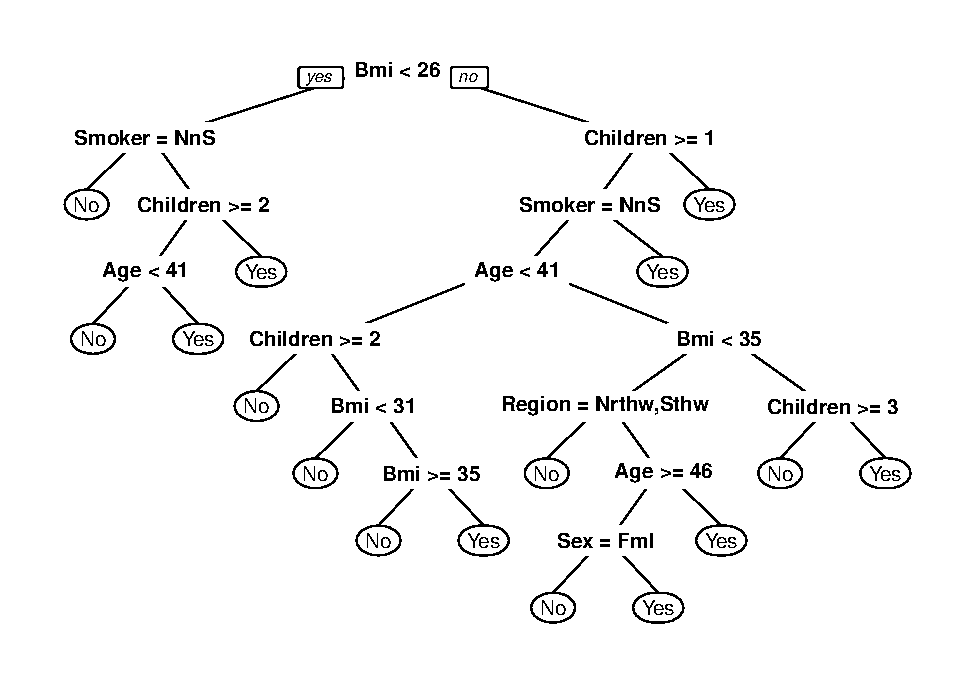
\includegraphics{2_Classification_Model_files/figure-latex/unnamed-chunk-7-1.pdf}

\begin{Shaded}
\begin{Highlighting}[]
\CommentTok{#Memvisualisasikan Decison Tree dengan lebih informatif}
\KeywordTok{fancyRpartPlot}\NormalTok{(tree)}
\end{Highlighting}
\end{Shaded}

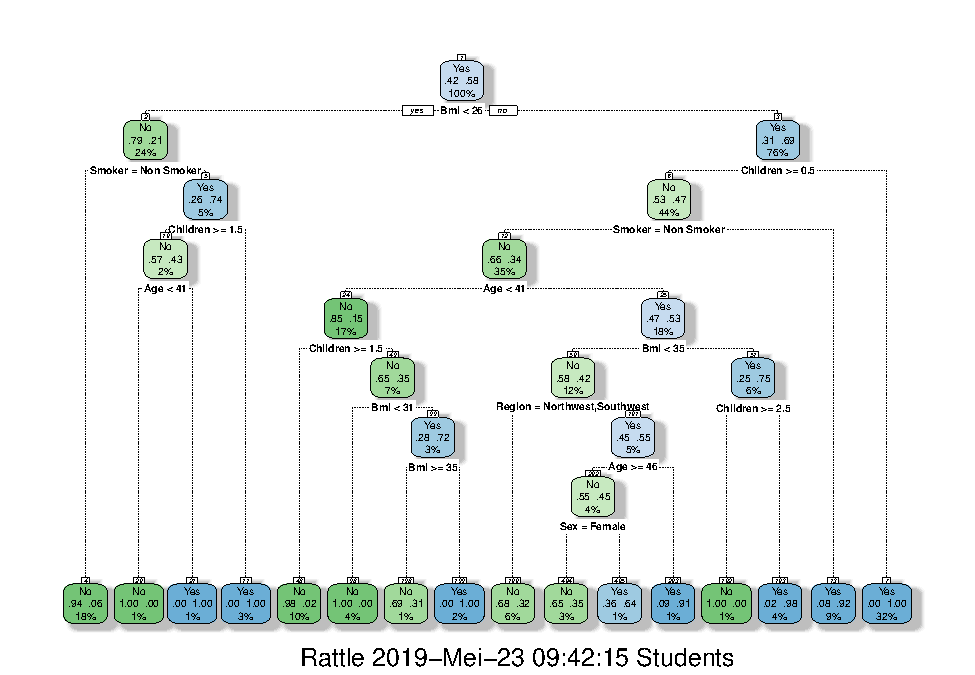
\includegraphics{2_Classification_Model_files/figure-latex/unnamed-chunk-8-1.pdf}

\begin{Shaded}
\begin{Highlighting}[]
\CommentTok{#Menggunakan Untuk Melakukan Prediksi Pada Data Testing}
\NormalTok{prediction <-}\StringTok{ }\KeywordTok{predict}\NormalTok{(tree, test, }\DataTypeTok{type =} \StringTok{"class"}\NormalTok{)}
\end{Highlighting}
\end{Shaded}

\hypertarget{validation}{%
\subsubsection{Validation}\label{validation}}

\begin{Shaded}
\begin{Highlighting}[]
\CommentTok{#Validasi Menggunakan Confussion Matrix}
\NormalTok{conf <-}\StringTok{ }\KeywordTok{table}\NormalTok{(test}\OperatorTok{$}\NormalTok{Claim, prediction)}
\NormalTok{conf}
\end{Highlighting}
\end{Shaded}

\begin{verbatim}
##      prediction
##        No Yes
##   No  146  13
##   Yes  32 211
\end{verbatim}

\begin{Shaded}
\begin{Highlighting}[]
\NormalTok{TP <-}\StringTok{ }\NormalTok{conf[}\DecValTok{1}\NormalTok{, }\DecValTok{1}\NormalTok{] }
\NormalTok{FN <-}\StringTok{ }\NormalTok{conf[}\DecValTok{1}\NormalTok{, }\DecValTok{2}\NormalTok{] }
\NormalTok{FP <-}\StringTok{ }\NormalTok{conf[}\DecValTok{2}\NormalTok{, }\DecValTok{1}\NormalTok{] }
\NormalTok{TN <-}\StringTok{ }\NormalTok{conf[}\DecValTok{2}\NormalTok{, }\DecValTok{2}\NormalTok{] }
\end{Highlighting}
\end{Shaded}

\begin{Shaded}
\begin{Highlighting}[]
\CommentTok{#Menghitung Nilai Akurasi}
\NormalTok{acc <-}\StringTok{ }\NormalTok{(TP }\OperatorTok{+}\StringTok{ }\NormalTok{TN)}\OperatorTok{/}\NormalTok{(TP }\OperatorTok{+}\StringTok{ }\NormalTok{FN }\OperatorTok{+}\StringTok{ }\NormalTok{FP }\OperatorTok{+}\StringTok{ }\NormalTok{TN)}
\NormalTok{accdt <-}\StringTok{ }\NormalTok{acc}
\NormalTok{acc}
\end{Highlighting}
\end{Shaded}

\begin{verbatim}
## [1] 0.8880597
\end{verbatim}

\begin{Shaded}
\begin{Highlighting}[]
\CommentTok{#Menghitung Nilai Precision}
\NormalTok{prec <-}\StringTok{ }\NormalTok{TP }\OperatorTok{/}\StringTok{ }\NormalTok{(TP }\OperatorTok{+}\StringTok{ }\NormalTok{FP)}
\NormalTok{prec}
\end{Highlighting}
\end{Shaded}

\begin{verbatim}
## [1] 0.8202247
\end{verbatim}

\begin{Shaded}
\begin{Highlighting}[]
\CommentTok{#Menghitung Nilai Recall}
\NormalTok{rec <-}\StringTok{ }\NormalTok{TP }\OperatorTok{/}\StringTok{ }\NormalTok{(TP }\OperatorTok{+}\StringTok{ }\NormalTok{FN)}
\NormalTok{rec}
\end{Highlighting}
\end{Shaded}

\begin{verbatim}
## [1] 0.918239
\end{verbatim}

\hypertarget{naive-bayes}{%
\subsection{Naive Bayes}\label{naive-bayes}}

\hypertarget{import-library-1}{%
\subsubsection{Import Library}\label{import-library-1}}

\begin{Shaded}
\begin{Highlighting}[]
\CommentTok{#Import Library}
\KeywordTok{library}\NormalTok{(naivebayes)}
\end{Highlighting}
\end{Shaded}

\begin{verbatim}
## Warning: package 'naivebayes' was built under R version 3.5.3
\end{verbatim}

\hypertarget{model-building-1}{%
\subsubsection{Model Building}\label{model-building-1}}

\begin{Shaded}
\begin{Highlighting}[]
\CommentTok{#Membuat model prediksi Naive Bayes}
\NormalTok{nb <-}\StringTok{ }\KeywordTok{naive_bayes}\NormalTok{(Claim }\OperatorTok{~}\StringTok{ }\NormalTok{., }\DataTypeTok{data =}\NormalTok{ train)}

\CommentTok{#Melihat model yang telah dibuat }
\NormalTok{nb}
\end{Highlighting}
\end{Shaded}

\begin{verbatim}
## ================================ Naive Bayes ================================= 
## Call: 
## naive_bayes.formula(formula = Claim ~ ., data = train)
## 
## A priori probabilities: 
## 
##        No       Yes 
## 0.4230769 0.5769231 
## 
## Tables: 
##       
## Age          No      Yes
##   mean 37.11111 40.51481
##   sd   12.44523 14.84770
## 
##         
## Sex             No       Yes
##   Female 0.5151515 0.4833333
##   Male   0.4848485 0.5166667
## 
##       
## Bmi           No       Yes
##   mean 27.990051 32.715269
##   sd    5.551262  5.723771
## 
##         
## Children        No       Yes
##     mean 1.7020202 0.6870370
##     sd   1.2292206 0.9935873
## 
##             
## Smoker              No       Yes
##   Non Smoker 0.9520202 0.6666667
##   Smoker     0.0479798 0.3333333
## 
## # ... and 2 more tables
\end{verbatim}

\begin{Shaded}
\begin{Highlighting}[]
\CommentTok{#Visualisasi Model}
\KeywordTok{par}\NormalTok{(}\DataTypeTok{mfrow=}\KeywordTok{c}\NormalTok{(}\DecValTok{2}\NormalTok{,}\DecValTok{4}\NormalTok{))}
\KeywordTok{plot}\NormalTok{(nb)}
\end{Highlighting}
\end{Shaded}

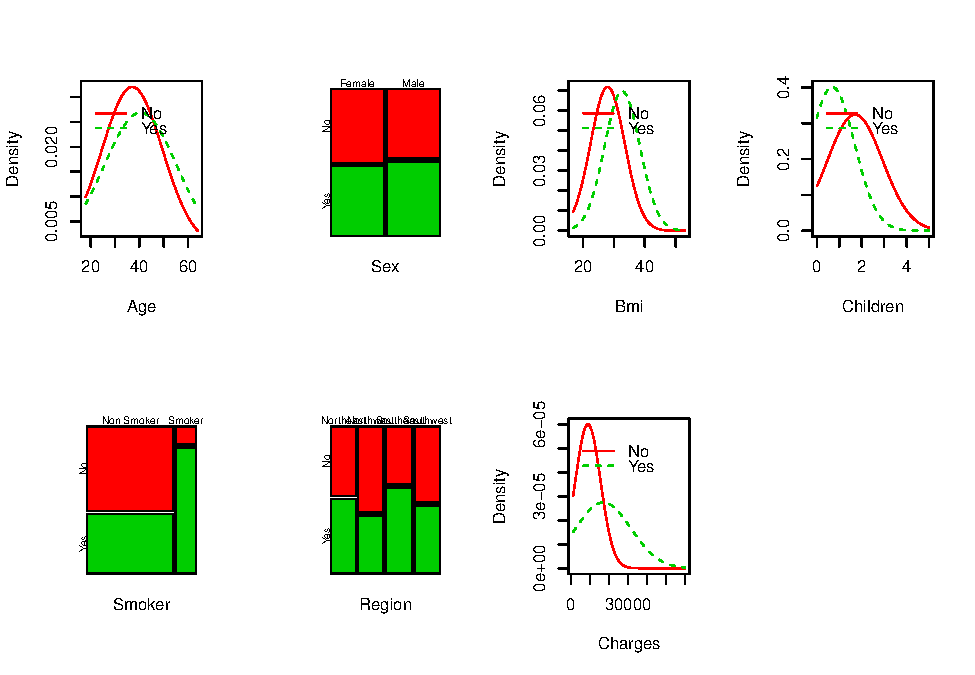
\includegraphics{2_Classification_Model_files/figure-latex/unnamed-chunk-17-1.pdf}

\begin{Shaded}
\begin{Highlighting}[]
\CommentTok{#Melakukan prediksi dengan data testing}
\NormalTok{pred_nb <-}\StringTok{ }\KeywordTok{predict}\NormalTok{(nb, }\KeywordTok{as.data.frame}\NormalTok{(test))}
\end{Highlighting}
\end{Shaded}

\hypertarget{validation-1}{%
\subsubsection{Validation}\label{validation-1}}

\begin{Shaded}
\begin{Highlighting}[]
\CommentTok{#Membuat Confussion Matrix Naive Bayes}
\NormalTok{confnb <-}\StringTok{ }\KeywordTok{table}\NormalTok{(test}\OperatorTok{$}\NormalTok{Claim, pred_nb)}
\NormalTok{confnb}
\end{Highlighting}
\end{Shaded}

\begin{verbatim}
##      pred_nb
##        No Yes
##   No  137  22
##   Yes  74 169
\end{verbatim}

\begin{Shaded}
\begin{Highlighting}[]
\NormalTok{TPn <-}\StringTok{ }\NormalTok{confnb[}\DecValTok{1}\NormalTok{, }\DecValTok{1}\NormalTok{] }
\NormalTok{FNn <-}\StringTok{ }\NormalTok{confnb[}\DecValTok{1}\NormalTok{, }\DecValTok{2}\NormalTok{] }
\NormalTok{FPn <-}\StringTok{ }\NormalTok{confnb[}\DecValTok{2}\NormalTok{, }\DecValTok{1}\NormalTok{] }
\NormalTok{TNn <-}\StringTok{ }\NormalTok{confnb[}\DecValTok{2}\NormalTok{, }\DecValTok{2}\NormalTok{] }
\end{Highlighting}
\end{Shaded}

\begin{Shaded}
\begin{Highlighting}[]
\CommentTok{#Menghitung Nilai Akurasi}
\NormalTok{accnb <-}\StringTok{ }\NormalTok{(TPn }\OperatorTok{+}\StringTok{ }\NormalTok{TNn)}\OperatorTok{/}\NormalTok{(TPn }\OperatorTok{+}\StringTok{ }\NormalTok{FNn }\OperatorTok{+}\StringTok{ }\NormalTok{FPn }\OperatorTok{+}\StringTok{ }\NormalTok{TNn)}
\NormalTok{accnb}
\end{Highlighting}
\end{Shaded}

\begin{verbatim}
## [1] 0.761194
\end{verbatim}

\begin{Shaded}
\begin{Highlighting}[]
\CommentTok{#Menghitung Nilai Precision}
\NormalTok{precnb <-}\StringTok{ }\NormalTok{TPn }\OperatorTok{/}\StringTok{ }\NormalTok{(TPn }\OperatorTok{+}\StringTok{ }\NormalTok{FPn)}
\NormalTok{precnb}
\end{Highlighting}
\end{Shaded}

\begin{verbatim}
## [1] 0.6492891
\end{verbatim}

\begin{Shaded}
\begin{Highlighting}[]
\CommentTok{#Menghitung Nilai Recall}
\NormalTok{recnb <-}\StringTok{ }\NormalTok{TPn }\OperatorTok{/}\StringTok{ }\NormalTok{(TPn }\OperatorTok{+}\StringTok{ }\NormalTok{FNn)}
\NormalTok{recnb}
\end{Highlighting}
\end{Shaded}

\begin{verbatim}
## [1] 0.8616352
\end{verbatim}

\hypertarget{k-nn}{%
\section{K-NN}\label{k-nn}}

\hypertarget{import-library-2}{%
\subsubsection{Import Library}\label{import-library-2}}

\begin{Shaded}
\begin{Highlighting}[]
\CommentTok{#import library yang dibutuhkan}
\KeywordTok{library}\NormalTok{(class)}
\KeywordTok{library}\NormalTok{(tidyverse)}
\end{Highlighting}
\end{Shaded}

\begin{verbatim}
## Warning: package 'tidyverse' was built under R version 3.5.3
\end{verbatim}

\begin{verbatim}
## -- Attaching packages ------ tidyverse 1.2.1 --
\end{verbatim}

\begin{verbatim}
## v ggplot2 3.1.1     v purrr   0.3.2
## v tibble  2.1.1     v dplyr   0.8.1
## v tidyr   0.8.3     v stringr 1.4.0
## v readr   1.3.1     v forcats 0.4.0
\end{verbatim}

\begin{verbatim}
## Warning: package 'ggplot2' was built under R version 3.5.3
\end{verbatim}

\begin{verbatim}
## Warning: package 'tibble' was built under R version 3.5.3
\end{verbatim}

\begin{verbatim}
## Warning: package 'tidyr' was built under R version 3.5.3
\end{verbatim}

\begin{verbatim}
## Warning: package 'readr' was built under R version 3.5.3
\end{verbatim}

\begin{verbatim}
## Warning: package 'purrr' was built under R version 3.5.3
\end{verbatim}

\begin{verbatim}
## Warning: package 'dplyr' was built under R version 3.5.3
\end{verbatim}

\begin{verbatim}
## Warning: package 'stringr' was built under R version 3.5.3
\end{verbatim}

\begin{verbatim}
## Warning: package 'forcats' was built under R version 3.5.3
\end{verbatim}

\begin{verbatim}
## -- Conflicts --------- tidyverse_conflicts() --
## x dplyr::filter() masks skimr::filter(), stats::filter()
## x dplyr::lag()    masks stats::lag()
\end{verbatim}

\hypertarget{data-pre-processing}{%
\subsubsection{Data Pre-Processing}\label{data-pre-processing}}

\begin{Shaded}
\begin{Highlighting}[]
\CommentTok{#Mengubah Data Ke Tipe Numerik}
\NormalTok{insurance1 <-}\StringTok{ }\NormalTok{insurance }\OperatorTok\StringTok{ }\KeywordTok{mutate_if}\NormalTok{(is.factor, as.numeric)}
\end{Highlighting}
\end{Shaded}

\begin{Shaded}
\begin{Highlighting}[]
\CommentTok{#Membuat fungsi Normalisasi}
\NormalTok{normalize<-}\ControlFlowTok{function}\NormalTok{(x)\{}
\NormalTok{  temp<-(x}\OperatorTok{-}\KeywordTok{min}\NormalTok{(x))}\OperatorTok{/}\NormalTok{(}\KeywordTok{max}\NormalTok{(x)}\OperatorTok{-}\KeywordTok{min}\NormalTok{(x))}
  \KeywordTok{return}\NormalTok{(temp)}
\NormalTok{\}}
\end{Highlighting}
\end{Shaded}

\begin{Shaded}
\begin{Highlighting}[]
\CommentTok{#Melakukan Normalisasi}
\NormalTok{kinsurance_n<-}\KeywordTok{as.data.frame}\NormalTok{(}\KeywordTok{lapply}\NormalTok{(insurance1[,}\KeywordTok{c}\NormalTok{(}\DecValTok{1}\OperatorTok{:}\DecValTok{7}\NormalTok{)],normalize))}
\end{Highlighting}
\end{Shaded}

\begin{Shaded}
\begin{Highlighting}[]
\CommentTok{#Membagi ke Data Train dan Data Testing}
\NormalTok{index_train <-}\StringTok{ }\KeywordTok{sample}\NormalTok{(}\DecValTok{1}\OperatorTok{:}\KeywordTok{nrow}\NormalTok{(kinsurance_n), }\FloatTok{0.7} \OperatorTok{*}\StringTok{ }\KeywordTok{nrow}\NormalTok{(kinsurance_n))}
\NormalTok{kinsurance_train <-}\StringTok{ }\NormalTok{kinsurance_n[index_train, ]}
\NormalTok{kinsurance_test <-}\StringTok{ }\NormalTok{kinsurance_n[}\OperatorTok{-}\NormalTok{index_train, ]}
\end{Highlighting}
\end{Shaded}

\begin{Shaded}
\begin{Highlighting}[]
\CommentTok{#Mengambil Label}
\NormalTok{kinsurance_train_target<-insurance1[index_train,}\DecValTok{8}\NormalTok{]}
\NormalTok{kinsurance_test_target<-insurance1[}\OperatorTok{-}\NormalTok{index_train, }\DecValTok{8}\NormalTok{]}
\end{Highlighting}
\end{Shaded}

\hypertarget{model-building-2}{%
\subsubsection{Model Building}\label{model-building-2}}

\begin{Shaded}
\begin{Highlighting}[]
\CommentTok{#Membuat KNN-Model dengan Nilai K=2}
\NormalTok{knnmodel <-}\KeywordTok{knn}\NormalTok{(}\DataTypeTok{train=}\NormalTok{kinsurance_train,}\DataTypeTok{test=}\NormalTok{kinsurance_test,}\DataTypeTok{cl=}\NormalTok{kinsurance_train_target,}\DataTypeTok{k=}\DecValTok{2}\NormalTok{)}
\end{Highlighting}
\end{Shaded}

\hypertarget{validation-2}{%
\subsubsection{Validation}\label{validation-2}}

\begin{Shaded}
\begin{Highlighting}[]
\CommentTok{#Validasi Menggunakan Confussion Matrix}
\NormalTok{confknn <-}\StringTok{ }\KeywordTok{table}\NormalTok{(kinsurance_test_target, knnmodel)}
\NormalTok{confknn}
\end{Highlighting}
\end{Shaded}

\begin{verbatim}
##                       knnmodel
## kinsurance_test_target   1   2
##                      1 124  31
##                      2  28 219
\end{verbatim}

\begin{Shaded}
\begin{Highlighting}[]
\NormalTok{TPk <-}\StringTok{ }\NormalTok{confknn[}\DecValTok{1}\NormalTok{, }\DecValTok{1}\NormalTok{] }
\NormalTok{FNk <-}\StringTok{ }\NormalTok{confknn[}\DecValTok{1}\NormalTok{, }\DecValTok{2}\NormalTok{] }
\NormalTok{FPk <-}\StringTok{ }\NormalTok{confknn[}\DecValTok{2}\NormalTok{, }\DecValTok{1}\NormalTok{] }
\NormalTok{TNk <-}\StringTok{ }\NormalTok{confknn[}\DecValTok{2}\NormalTok{, }\DecValTok{2}\NormalTok{]}
\end{Highlighting}
\end{Shaded}

\begin{Shaded}
\begin{Highlighting}[]
\CommentTok{#Melihat Nilai Akurasi K-NN}
\NormalTok{acck <-}\StringTok{ }\NormalTok{(TPk }\OperatorTok{+}\StringTok{ }\NormalTok{TNk)}\OperatorTok{/}\NormalTok{(TPk }\OperatorTok{+}\StringTok{ }\NormalTok{FNk }\OperatorTok{+}\StringTok{ }\NormalTok{FPk }\OperatorTok{+}\StringTok{ }\NormalTok{TNk)}
\NormalTok{acck}
\end{Highlighting}
\end{Shaded}

\begin{verbatim}
## [1] 0.8532338
\end{verbatim}

\begin{Shaded}
\begin{Highlighting}[]
\CommentTok{#Melihat Nilai Precision K-NN}
\NormalTok{preck <-}\StringTok{ }\NormalTok{TPk }\OperatorTok{/}\StringTok{ }\NormalTok{(TPk }\OperatorTok{+}\StringTok{ }\NormalTok{FPk)}
\NormalTok{preck}
\end{Highlighting}
\end{Shaded}

\begin{verbatim}
## [1] 0.8157895
\end{verbatim}

\begin{Shaded}
\begin{Highlighting}[]
\CommentTok{#Melihat Nilai Recall K-NN}
\NormalTok{reck <-}\StringTok{ }\NormalTok{TPk }\OperatorTok{/}\StringTok{ }\NormalTok{(TPk }\OperatorTok{+}\StringTok{ }\NormalTok{FNk)}
\NormalTok{reck}
\end{Highlighting}
\end{Shaded}

\begin{verbatim}
## [1] 0.8
\end{verbatim}

\hypertarget{model-comparison}{%
\subsection{Model Comparison}\label{model-comparison}}

\begin{Shaded}
\begin{Highlighting}[]
\CommentTok{#Nilai Akurasi Decision Tree}
\NormalTok{accdt}
\end{Highlighting}
\end{Shaded}

\begin{verbatim}
## [1] 0.8880597
\end{verbatim}

\begin{Shaded}
\begin{Highlighting}[]
\CommentTok{#Nilai Akurasi Naive Bayes}
\NormalTok{accnb}
\end{Highlighting}
\end{Shaded}

\begin{verbatim}
## [1] 0.761194
\end{verbatim}

\begin{Shaded}
\begin{Highlighting}[]
\CommentTok{#Nilai Akurasi K-NN}
\NormalTok{acck}
\end{Highlighting}
\end{Shaded}

\begin{verbatim}
## [1] 0.8532338
\end{verbatim}


\end{document}
